\documentclass[hyperref={unicode}]{beamer}
\usepackage{CJKutf8}
\usepackage{color}
\usepackage{graphicx}
\usepackage{wrapfig}
\usepackage{hyperref}
\usetheme{Madrid}
%\usetheme{Warsaw}
%\usetheme{Singapore}
%\usetheme{Berlin}
\usecolortheme{whale}
% don't need for Madrid, but others need.
% \useoutertheme{infolines} 
% Adding footnotes
\usepackage[absolute,overlay]{textpos} 
\newenvironment{reference}[2]{% 
  \begin{textblock*}{\textwidth}(#1,#2) 
      \footnotesize\it\bgroup\color{red!50!black}}{\egroup\end{textblock*}} 
% changing the itemization markers
\setbeamertemplate{items}[ball]

% Rounder boxes and shadows
\setbeamertemplate{blocks}[rounded][shadow=true]
% Getting rid of the nabigation icons
\setbeamertemplate{navigation symbols}{}
\begin{document}
\begin{CJK}{UTF8}{gkai}
\title{人机互动: 智能机器人的智能问题研究}
\subtitle{AI Course Presentation}
\author{李晓东}
% \date{\today}
\renewcommand{\today}{ April 6, 2012}
\institute{大连理工大学软件学院}

\logo{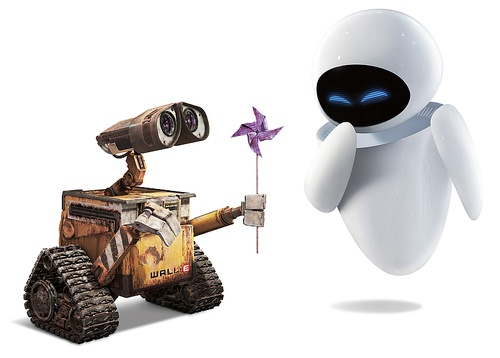
\includegraphics[width=1cm, height=1cm]{logo1}}
\begin{frame}
  \titlepage
\end{frame}
% automatically print the table of contents  at the beginning of each
% section and subsection.
\AtBeginSection[]
{
  \begin{frame}
    \tableofcontents[currentsection,currentsubsection]
  \end{frame}
}

\section{中国}
\begin{frame}{Splitting a slide into columns}

The line you are reading goes all the way across the slide.
From the left margin to the right margin.  Now we are going
to split the slide into two columns.
\bigskip

\begin{columns}
  \begin{column}{0.5\textwidth}
    Here is the first column.  We put an itemized list in it.
    \begin{itemize}
      \item This is an item
      \item This is another item
      \item Yet another item
    \end{itemize}
  \end{column}

  \begin{column}{0.3\textwidth}
    Here is the second column.  We will put a picture in it.
    %\centerline{\includegraphics[width=0.7\textwidth]{image2.png}}
  \end{column}
\end{columns}
\bigskip
The line you are reading goes all the way across the slide.
From the left margin to the right margin.
\end{frame}

\section{中国人}
\begin{frame}{Footnote example}
   \begin{reference}{4mm}{85mm}
       V. Jikov, S. Kozlov and O. Olenik, Homogenization
       of differential operators and integral
       functionals, Springer, 1994.
   \end{reference} 
  
   This is a test.
\end{frame}

\section{我们爱我们的祖国}
\begin{frame}{中国万岁}
\begin{block}{长城}
  \begin{itemize}
  \item   The Great Wall 
  \item  The Great Fire Wall
  \item F**k
  \end{itemize}
\end{block}  
\end{frame}

\section{Color}
\begin{frame}{Color Demo}
  \textcolor{blue}{This text is in blue} \\
  % Text background color is set using the \colorbox command.
  \colorbox{yellow}{This text is highlighted in yellow}  \\

  % combine various color and font elements to achive interesting results
  \colorbox{yellow}{ 
    \textcolor{red}{ 
        \textbf{ 
            Bold text in red, highlighted in yellow 
        } 
    } 
} 

% To encose text in a bordered box:
\fcolorbox{red}{yellow}{A yellow box with red border} 

% set border's thickness
\setlength{\fboxrule}{4pt} 
\fcolorbox{red}{white}{A white box with a red border of thickness 4 points} 

\setlength{\fboxrule}{4pt} 
\setlength{\fboxsep}{0pt} 
\fcolorbox{red}{white}{A white box with a red border and separation of 0 points}

\end{frame}

\section{The end}
\begin{frame}{Q\&A}
  \begin{center}
    \LARGE{\alert{Thanks!}}
  \end{center}
\end{frame}

\end{CJK}
\end{document}
